\documentclass[10pt]{article}
\usepackage[margin=0.72in]{geometry}
\usepackage[T1]{fontenc}
\usepackage{libertinus}
\usepackage{microtype}
\usepackage{enumitem}
\usepackage{xcolor}
\usepackage{titlesec}
\usepackage{booktabs}
\usepackage{tabularx}
\usepackage{graphicx}
\usepackage{pifont}
\definecolor{rule}{RGB}{120,30,30}
\definecolor{sered}{RGB}{200,0,0}
\newcommand{\se}[1]{\textcolor{sered}{#1}}
\usepackage{draftwatermark}
\SetWatermarkText{WORK IN PROGRESS}
\SetWatermarkScale{0.45}
\SetWatermarkColor{gray!18}
\titleformat{\section}{\large\bfseries\color{rule}}{}{0pt}{}
\titlespacing*{\section}{0pt}{5pt}{2pt}
\setlist{nosep,leftmargin=1.2em}
\pagestyle{empty}
\setlength{\parindent}{0pt}
\setlength{\parskip}{2.5pt}
\linespread{0.98}

\begin{document}

{\large\bfseries AI at CSC: Situation and Way Forward}\\[1pt]
{\small To: CSC leadership \quad From: Tim Menzies \quad August 2026 \quad (one page + four one-page appendices)}

\vspace{2pt}\textcolor{rule}{\hrule height 1pt}

{\small\emph{This memo is based on a preliminary analysis of our subjects. If there is interest in moving forward, that analysis must be carefully verified --- e.g., by discussing this memo with the lecturers of those subjects and with other interested parties.}}

\section{Part 1 --- Where we stand, and the way forward}

\textbf{Three blunt facts.}
\begin{enumerate}
\item \textbf{Peers ship while we deliberate.} Purdue: BS in AI. Arizona: BS + minor. Georgia Tech: two AI minors and an NVIDIA-backed Makerspace. Duke: required AI in the CS core this fall. Maryland: BS/BA in AI, 2026--27. NC~State: no minor, no standalone credential, BS ``on hold.'' The bottleneck is our own process, not our talent.
\item \textbf{Industry hiring has changed --- and industry disagrees on how.} Our advisory-board interviews show wide divergence. Some CTOs push to remove the human: ``If the human is in the loop, you are going too slow.'' Others want better humans: ``We want to hire, not so much your degree, but someone who is a problem solver --- everything will be moving fast.'' The remove-the-human camp rides today's gold rush of cheap, subsidized tokens --- perhaps to its detriment. Both camps need what we teach: people who can build \emph{and check} agentic systems, not merely operate them.
\item \textbf{Current AI economics will not hold.} Token and GPU costs climb, vendors ration capacity, and many AI products lose money per user. If (when) the bubble bursts, the field moves to a new era of cost-effective neurosymbolic AI: mix and match the best of LLMs with cheaper, faster methods. That era is our opening, not only a threat --- it is the curriculum we can own (see Part~2).
\end{enumerate}

\textbf{The way forward, ranked by friction (lowest first).}
\begin{enumerate}
\item \textbf{Now:} add AI-assessment learning objectives to existing courses (Appendices A--D) --- course-level edits, no degree paperwork.
\item \textbf{This semester:} land MS+AI (already near approval) and launch CSC~202/301 as the college-wide freshman AI sequence. Service enrollment funds staff lines; degrees follow money.
\item \textbf{Next:} AI minor. Park the BS --- the ``on hold'' fight is not winnable this year, and everything above proceeds without it.
\end{enumerate}

\textbf{NC State goals already exists in print.} Every step above executes Provost Pfaendtner's published agenda (Red Hat Research Quarterly, Summer 2026). From our repertory-grid study of NCSU CSC against the 12 BOG-approved peers plus Duke: nine constructs (C1--C9), each derived from the Provost's published positions, each department scored 1 (ideal) to 5 with per-cell public evidence (full grid on request; Purdue closest to the ideal, NCSU one point back with Duke and Georgia). Below, each construct with the Provost's own words and the outcomes (Appendices A and C) that serve it.

\vspace{2pt}
{\scriptsize\renewcommand{\arraystretch}{0.95}%
\begin{tabularx}{\textwidth}{@{}l X l@{}}
\toprule
\textbf{Construct (ideal pole)} & \textbf{The Provost, in print} & \textbf{Outcomes}\\
\midrule
C1 AI dosed early, redosed often & ``Where does the dose of AI come early on, and where do we keep redosing it?'' & 1--5, 8, 18, 20\\
C2 Fundamentals-first & ``You can't replace the time and space a college student has to learn fundamentals and critical thinking.'' & all 22\\
C3 Parsimony: small, cheap models & ``Small language models that do bespoke tasks with way less power usage\ldots transformational\ldots the way we educate.'' & 8, 9, 22\\
C4 Doing, not talking & ``Stop talking, start doing.'' & all 22\\
C5 Open source \& reproducibility & ``Open source means we publish our work first.'' & 3, 16\\
C6 Faculty AI-upskilling & ``A faculty fellowship program\ldots with the explicit purpose of upskilling in AI.'' & 20\\
C7 Serves the whole college & ``1,850 brand-new freshmen\ldots how are we teaching them to think about AI?'' & 1--3, 8, 18, 20\\
C8 Ships credentials, agile & ``Being agile is essential.'' & 3, 8, 18, 20\\
C9 AI rigor: test/eval/secure AI & Asked about debugging and security fundamentals under AI: ``100\%.'' & 2, 3, 11--16, 19\\
\bottomrule
\end{tabularx}}

\section{Part 2 --- The merits of CS: why study CS/SE in the age of AI?}

\textbf{Tools get students hired; judgment gets them promoted.} AI now writes code cheaply. Someone still must define what correct means, verify generated claims, review work they did not write, secure the system, and measure cost against quality. Those are computer-science skills, and together they are the senior-engineer role --- exactly the role industry deskilling threatens to empty out. We train the reviewers, not the reviewed.

\textbf{CSC studies what others merely use.} Appendices A and C list twenty-two skills for \emph{assessing computation} that no other department teaches. Departments that use AI cannot repair its defects; the department that studies those defects must teach them --- to the whole college.

\textbf{Industry's ``durable skills'' are already in this set --- graded by artifact, not essay.} Employers ask for critical thinking, communication, collaboration, adaptability, leadership, and a growth mindset. The outcomes test each against evidence: critical thinking = defect reasons that survive challenge (4, 14, 18); communication = a second team acts on the work without asking a question (1, 11); collaboration = every stakeholder signs off (10, 17); adaptability and growth mindset = learn the next tool from documentation alone (14, 20); leadership = the MVP business case (10), the thinnest of the six.

\textbf{Our resource limits mirror industry's --- so we teach for them.} We will not win a GPU arms race, and neither will most employers. We therefore teach AI that does not require exponential compute: small models, hybrid neurosymbolic methods, rigorous evaluation on cheap hardware. Most of the appendix skills need no GPU at all. A curriculum built on judgment and parsimony survives an AI bubble; one built on unlimited tokens does not.

\newpage

{\large\bfseries Appendix A: Twenty-two skills for assessing computation, as learning outcomes --- undergraduate}\\[1pt]
{\small Skills that CS teaches and no one else does. Coverage column shows where the CSC undergraduate program touches each today: \textbf{ok} = covered; \emph{partial} = course exists but predates AI-generated systems; \textcolor{rule}{\textbf{gap}} = not taught. \se{Red course numbers} are SE subjects, including the proposed Fall~2026 UG SE concentration. Right columns: \emph{easy CPU} = teachable without intensive CPU/GPU; \emph{broad} = teachable across the whole university (no GPU, no budget, no programming prerequisite).}

\vspace{4pt}
\footnotesize
\begin{tabularx}{\textwidth}{@{}r X l @{\hspace{6pt}}c@{\hspace{6pt}}c@{}}
\toprule
& \textbf{Students will be able to\ldots} & \textbf{CSC ugrad today} & \rotatebox[origin=b]{60}{\textbf{easy CPU}} & \rotatebox[origin=b]{60}{\textbf{broad}}\\
\midrule
\multicolumn{5}{@{}l}{\emph{Is it right?}}\\
1 & Given a vague goal, specify a domain definition (inputs, outputs, correctness, out-of-scope) that a second team can test without asking a question. & \se{216}, \se{326} --- \emph{partial} & \ding{51} & \ding{51}\\
2 & Given a spec, design a test suite that detects all seeded defects, covering boundaries, regressions, and nondeterministic outputs. & \se{326}, \se{404} (new) --- \emph{partial} & \ding{51} & \ding{51}\\
3 & Given generated statistics, plots, or citations, verify each against raw data or the primary source; flag whatever cannot be traced. & \textcolor{rule}{\textbf{gap}} & \ding{51} & \ding{51}\\
4 & Given code they did not write, identify defects, judge maintainability, and accept or reject with reasons that survive challenge. & \se{326}, \se{421}, \se{491a} --- \emph{partial} & \ding{51} & \\
5 & Given an algorithm, prove its invariants and classify its problem as tractable, intractable, or undecidable. & 226, 333, 366 --- \textbf{ok} & \ding{51} & \\
\multicolumn{5}{@{}l}{\emph{What does it cost?}}\\
8 & Given an AI result, benchmark it against at least one non-AI baseline over at least 20 repeated runs, reporting effect size and variance. & \textcolor{rule}{\textbf{gap}} & \ding{51} & \ding{51}\\
9 & Given a decomposed workflow, allocate each sub-task to an LLM, retrieval, optimization, or deterministic logic, and defend the split with measured cost and quality. & \se{421}, \se{491a}, \se{491b} (electives) --- \emph{partial} & \ding{51} & \\
10 & Given conflicting stakeholder needs, produce an MVP scope and release plan with a business case that prices the do-nothing option. & \se{408} (elective) --- \emph{partial} & \ding{51} & \\
\multicolumn{5}{@{}l}{\emph{Can it be trusted?}}\\
11 & Given a system design, build a threat model --- assets, adversaries, attack surface --- so complete that a second team finds no critical item to add. & 405, 474 (electives) --- \textbf{ok} & \ding{51} & \\
12 & Given a deployed system, execute an adversarial test plan covering prompt injection, data leakage, and access weakness. & \se{415} --- \emph{partial} &  & \\
13 & Given a pipeline, audit training-data provenance, license status of generated code, and PII flow, and state what risk remains after the fixes. & 379, \se{433} --- \emph{partial} & \ding{51} & \\
14 & Given a failure, diagnose the fault mode and specify detection and recovery --- not a patch. & 246 --- \emph{partial} & \ding{51} & \\
15 & Given a model, evaluate it beyond accuracy --- calibration, robustness, fairness, drift --- reporting each against a stated threshold. & 422, 425 --- \emph{partial} &  & \\
16 & Given a published result, reproduce it from its stated environment, seeds, and scripts. & \textcolor{rule}{\textbf{gap}} &  & \\
\multicolumn{5}{@{}l}{\emph{Does it scale? --- up (larger problems), out (more users), down (edge devices)}}\\
6 & Given an algorithm, predict scaling from complexity analysis, then confirm by measurement. & 316, 366 --- \textbf{ok} & \ding{51} & \\
7 & Given a running system, measure latency, throughput, and run-to-run variance, and locate the bottleneck. & 230, 246 --- \emph{partial} & \ding{51} & \\
19 & Given a production system, design monitors for drift and a response plan for when they fire. & \textcolor{rule}{\textbf{gap}} &  & \\
21 & Given a deployed service, load-test at ten times the expected users, report cost per added user, and locate where latency breaks the stated service objective. & \textcolor{rule}{\textbf{gap}} &  & \\
22 & Given a fixed CPU and memory budget, shrink a model or system until it fits, and report the quality lost. & \textcolor{rule}{\textbf{gap}} &  & \\
\multicolumn{5}{@{}l}{\emph{Does it fit the world?}}\\
17 & Given stakeholders in conflict, elicit requirements and negotiate a release plan that every stakeholder signs off on. & \se{326}, \se{418} --- \textbf{ok} & \ding{51} & \\
18 & Given a hypothesis, design an experiment with controls, confounds handled, and ablations. & \textcolor{rule}{\textbf{gap}} & \ding{51} & \ding{51}\\
20 & Given only vendor documentation, reimplement a core abstraction in under 500 lines and evaluate it against the industrial version. & \se{491a} (elective) --- \emph{partial} & \ding{51} & \ding{51}\\
\bottomrule
\end{tabularx}

{\footnotesize Key --- outcomes keep their numbers when regrouped; 21--22 are new. Special-topics sections pending permanent numbers: \se{491a} = Secrets of the Software Gurus (proposed CSC 413); \se{491b} = SE for AI (proposed CSC 426); \se{404} = Software Testing (proposed, SE-concentration required core).}

\vspace{4pt}
\normalsize
\textbf{How the undergraduate program covers this set.} Four outcomes are solid (5, 6, 11, 17): algorithmic fundamentals, threat modeling, requirements --- our base, and no other department on campus has it. Seven are outright gaps. Five of those (3, 8, 16, 18, 19) are AI-facing \emph{assessment}: verifying generated claims, benchmarking against baselines, reproducing, experimenting, monitoring. The other two are the scale asks (21, 22): no course load-tests to many users, and none fits a system into an edge budget. The partials have a home course that predates generated code (e.g., 326 tests deterministic programs; 422/425 stop at accuracy). Every gap and partial is fixable by course-level learning-objective edits or by moving an elective (408, 421, 491a, 491b) toward the core --- no new degree, no new committee. Note how much of the table is \se{red}: the proposed SE concentration already routes students through most of the partials, so its learning-objective edits are the highest-leverage fix available. The \emph{broad} outcomes (1--3, 8, 18, 20) need no GPU, no budget, and no programming prerequisite: teachable to the whole College of Engineering this year. Sixteen of the twenty-two (\emph{easy CPU} column) need no intensive compute at all; only 12, 15, 16, 19, 21, and 22 require a live system, real models, or infrastructure.

\newpage

{\large\bfseries Appendix B: The undergraduate subjects, scored on the Provost's constructs}\\[1pt]
{\small A repertory grid over subjects, not departments. Elements: the 21 subjects that Appendix A cites, plus the Provost's ideal subject. Constructs: the nine constructs of our department study (table, page~1), reworded to subject level. Scale: 1 = the Provost's ideal pole, 5 = the contrast pole; d = distance from IDEAL. Scores come from the public catalog and the Appendix A analysis. They are preliminary. Each score must be checked with the lecturer.}

\vspace{-2pt}
\begin{center}
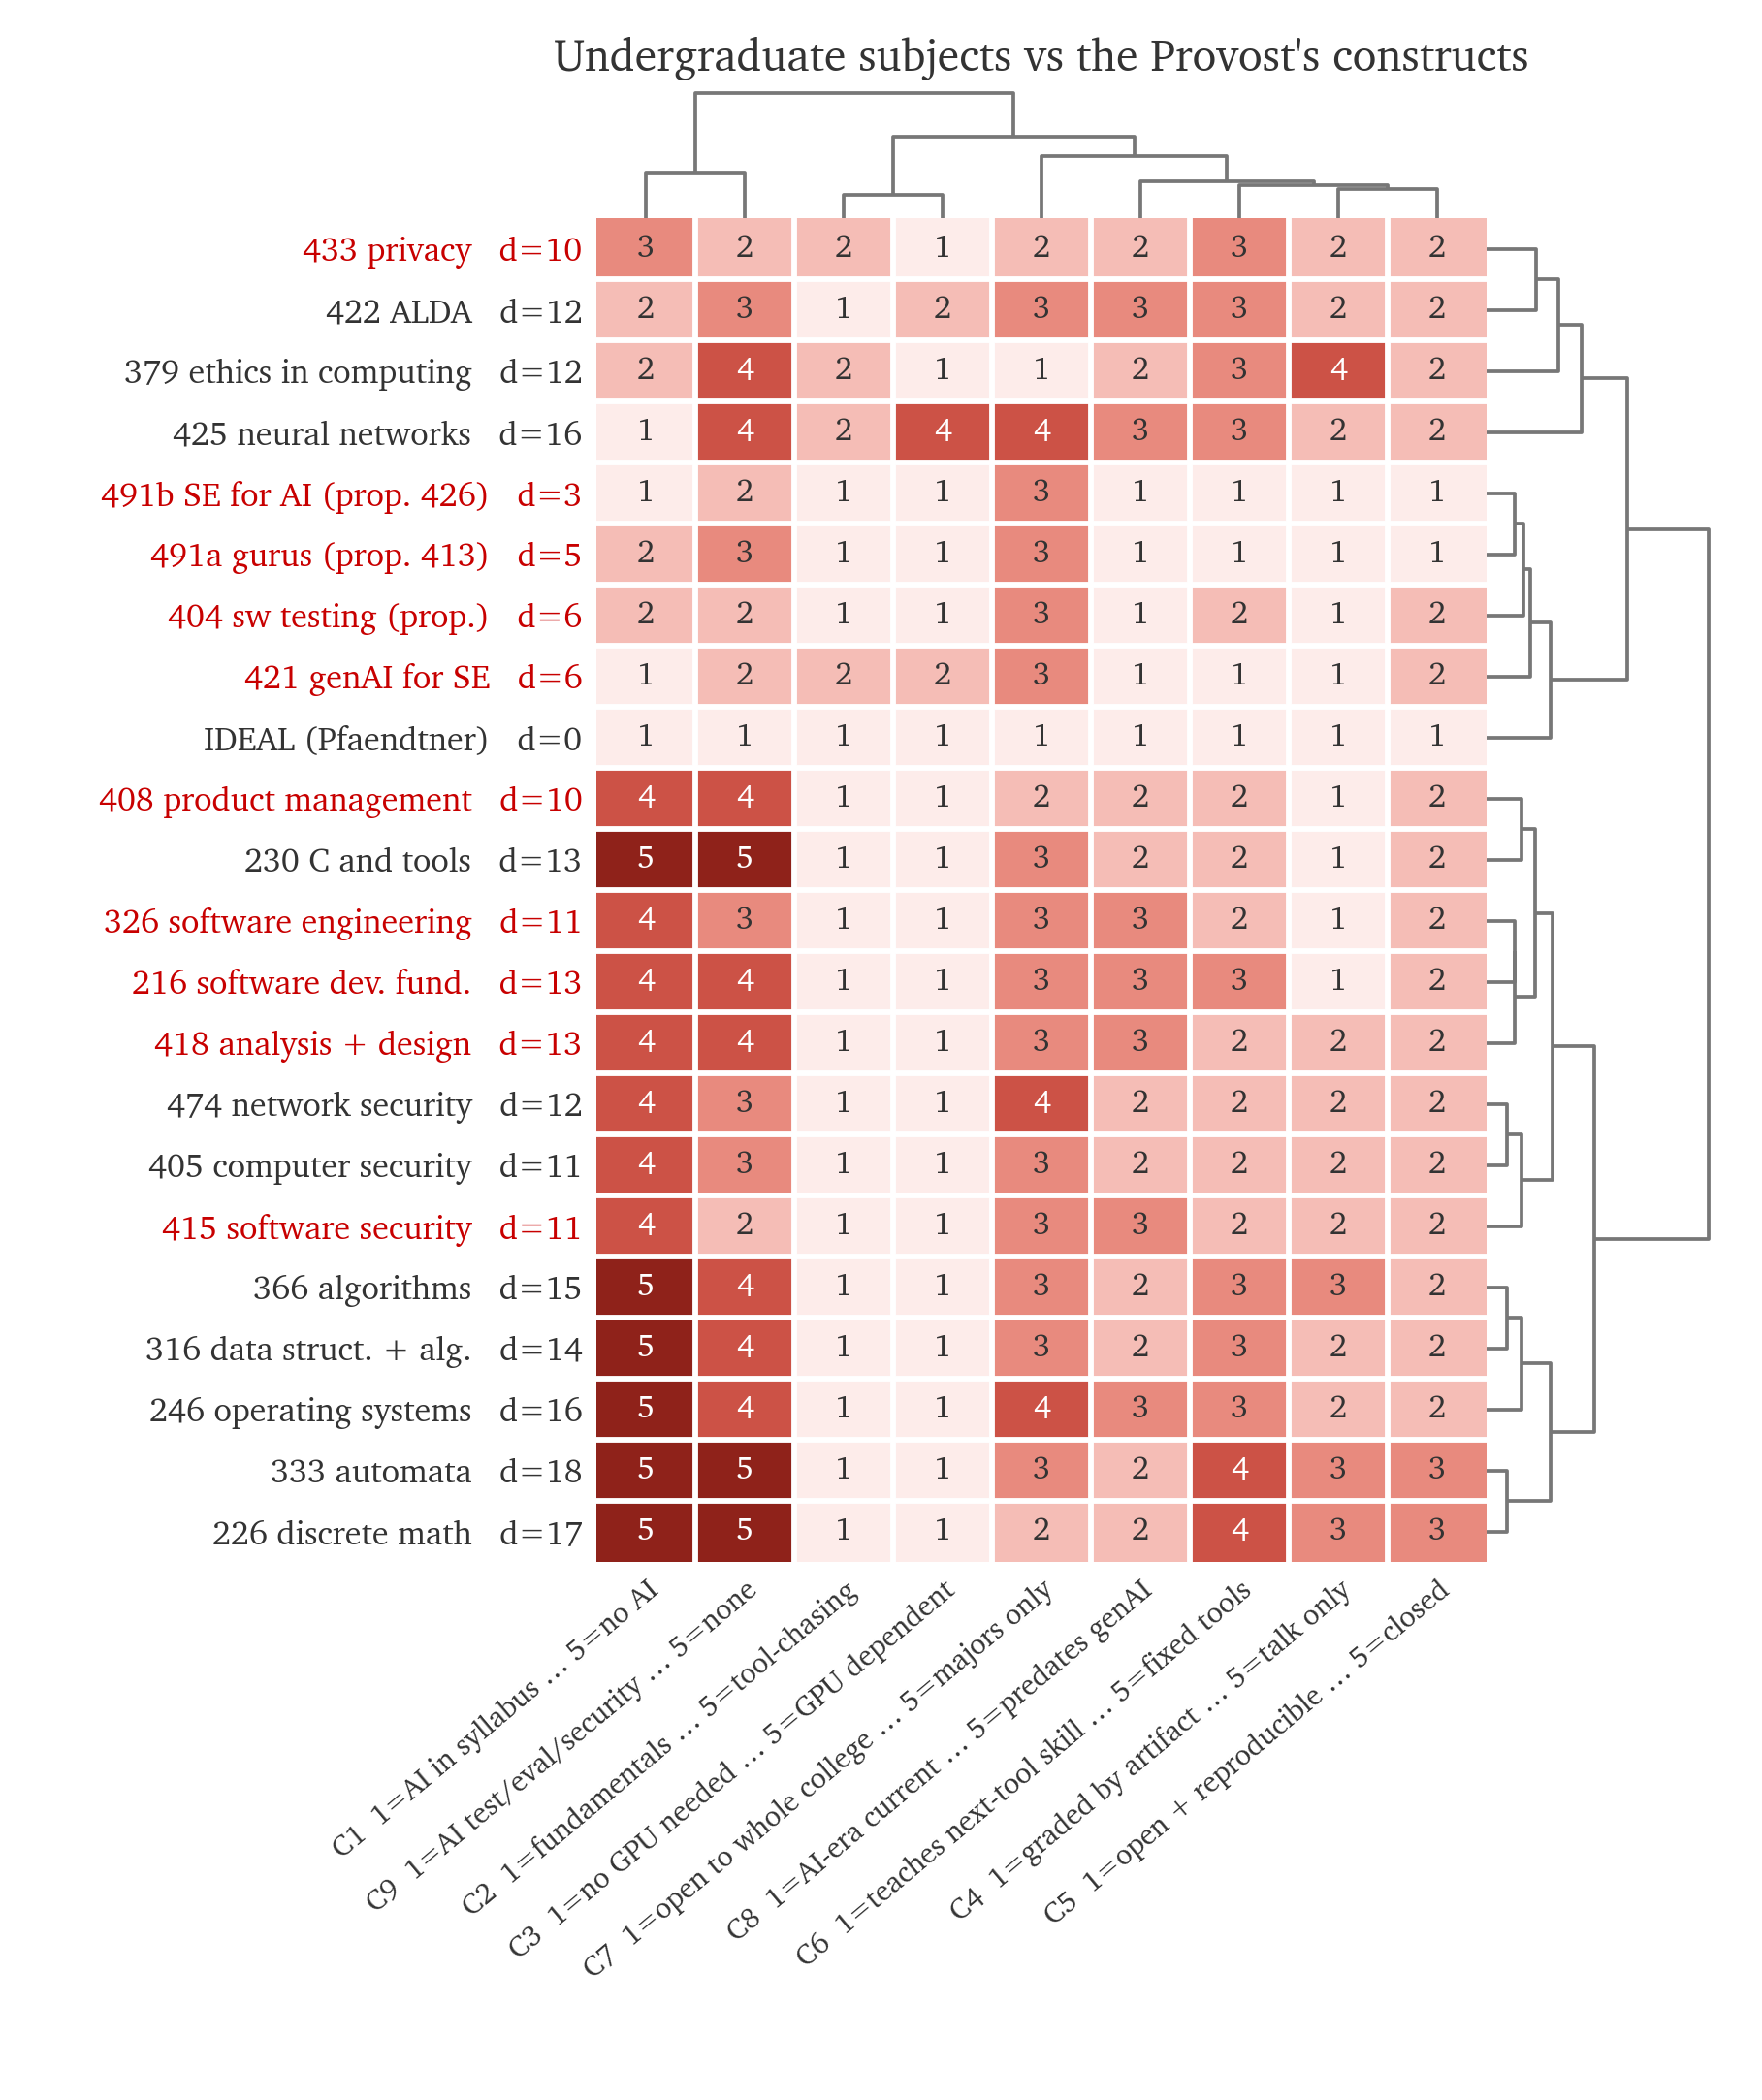
\includegraphics[width=0.68\textwidth]{ugrad-grid.png}
\end{center}
\vspace{-8pt}

{\footnotesize FOCUS-style clustered grid: dendrograms above (constructs) and right (subjects). \se{Red labels} are SE subjects.}

\textbf{Three reads.} \textbf{(i) The proposed SE courses cluster with the ideal.} The right-hand dendrogram puts \se{491b} (d=3), \se{491a} (d=5), \se{404} (d=6), and \se{421} (d=6) on the same branch as IDEAL. No other subject comes closer than d=10. The Fall 2026 SE concentration is not a side bet. It is the closest match to the Provost's wish list that this college owns. \textbf{(ii) For the theory core, distance is not deficiency.} The bottom cluster (226, 333, 246, 316, 366; d=14--18) scores a perfect 1 on fundamentals --- the one construct the Provost defends against deskilling. Its distance comes from two columns only: no AI in the syllabus (C1) and no AI assessment (C9). These subjects are not problems. They are the redose targets. \textbf{(iii) The C9 column is almost empty.} Outside the proposed courses, only \se{415} and \se{433} score 2 on AI test/eval/security. This is the same empty lane our department study found sector-wide (no peer scores better than 2 on C9), now located to the exact subjects that must fill it. One more column deserves note: C3 (no GPU needed) scores 1--2 everywhere except 425. Parsimony is already our default. We can teach the Provost's cheap-model agenda with the hardware we own.

\textbf{What the grid buys us.} The middle cluster (216, 230, 326, 405, 408, 415, 418, 474) is artifact-graded, GPU-free, and current on everything except AI. Each subject there sits 10--13 points from ideal, and almost all of that distance lives in C1 and C9. Course-level learning-objective edits --- an AI dose plus an AI-assessment outcome --- move each of them 4--6 points toward ideal with no degree paperwork.

\newpage

{\large\bfseries Appendix C: The same twenty-two outcomes --- graduate}\\[1pt]
{\small Same outcomes, mapped to the CSC graduate program. Identical objectives at both levels is deliberate: the skill does not change with level, the criterion does --- graduate students meet each criterion on larger systems, against stiffer thresholds, defended to research standard. Right columns as in Appendix A: \emph{easy CPU} = no intensive CPU/GPU; \emph{broad} = teachable university-wide. \se{Red course numbers} are SE subjects: graduate SE courses (510, 515, 517, 519) and the proposed graduate twins of dual-listed UG SE concentration courses (518, 521, 591b --- not yet in the catalog; see table key).}

\vspace{4pt}
\footnotesize
\begin{tabularx}{\textwidth}{@{}r X l @{\hspace{6pt}}c@{\hspace{6pt}}c@{}}
\toprule
& \textbf{Students will be able to\ldots} & \textbf{CSC grad today} & \rotatebox[origin=b]{60}{\textbf{easy CPU}} & \rotatebox[origin=b]{60}{\textbf{broad}}\\
\midrule
\multicolumn{5}{@{}l}{\emph{Is it right?}}\\
1 & Given a vague goal, specify a domain definition (inputs, outputs, correctness, out-of-scope) that a second team can test without asking a question. & \se{510}, \se{518} (prop.) --- \emph{partial} & \ding{51} & \ding{51}\\
2 & Given a spec, design a test suite that detects all seeded defects, covering boundaries, regressions, and nondeterministic outputs. & \se{510} --- \emph{partial} & \ding{51} & \ding{51}\\
3 & Given generated statistics, plots, or citations, verify each against raw data or the primary source; flag whatever cannot be traced. & \textcolor{rule}{\textbf{gap}} & \ding{51} & \ding{51}\\
4 & Given code they did not write, identify defects, judge maintainability, and accept or reject with reasons that survive challenge. & \se{510}, \se{517}, \se{521} (prop.) --- \emph{partial} & \ding{51} & \\
5 & Given an algorithm, prove its invariants and classify its problem as tractable, intractable, or undecidable. & 505, 512 --- \textbf{ok} & \ding{51} & \\
\multicolumn{5}{@{}l}{\emph{What does it cost?}}\\
8 & Given an AI result, benchmark it against at least one non-AI baseline over at least 20 repeated runs, reporting effect size and variance. & 522 (labs, light) --- \emph{partial} & \ding{51} & \ding{51}\\
9 & Given a decomposed workflow, allocate each sub-task to an LLM, retrieval, optimization, or deterministic logic, and defend the split with measured cost and quality. & \se{591b}, 528 --- \emph{partial} & \ding{51} & \\
10 & Given conflicting stakeholder needs, produce an MVP scope and release plan with a business case that prices the do-nothing option. & \se{510} --- \emph{partial} & \ding{51} & \\
\multicolumn{5}{@{}l}{\emph{Can it be trusted?}}\\
11 & Given a system design, build a threat model --- assets, adversaries, attack surface --- so complete that a second team finds no critical item to add. & \se{515}, 537 --- \textbf{ok} & \ding{51} & \\
12 & Given a deployed system, execute an adversarial test plan covering prompt injection, data leakage, and access weakness. & \se{515}, 537 --- \emph{partial} &  & \\
13 & Given a pipeline, audit training-data provenance, license status of generated code, and PII flow, and state what risk remains after the fixes. & 533, 534 --- \emph{partial} & \ding{51} & \\
14 & Given a failure, diagnose the fault mode and specify detection and recovery --- not a patch. & 501, 537 --- \emph{partial} & \ding{51} & \\
15 & Given a model, evaluate it beyond accuracy --- calibration, robustness, fairness, drift --- reporting each against a stated threshold. & 528 --- \textbf{ok} (elective) &  & \\
16 & Given a published result, reproduce it from its stated environment, seeds, and scripts. & \se{519} --- \emph{partial} &  & \\
\multicolumn{5}{@{}l}{\emph{Does it scale? --- up (larger problems), out (more users), down (edge devices)}}\\
6 & Given an algorithm, predict scaling from complexity analysis, then confirm by measurement. & 505, 572 --- \textbf{ok} & \ding{51} & \\
7 & Given a running system, measure latency, throughput, and run-to-run variance, and locate the bottleneck. & 501 --- \emph{partial} & \ding{51} & \\
19 & Given a production system, design monitors for drift and a response plan for when they fire. & \se{519} (light) --- \emph{partial} &  & \\
21 & Given a deployed service, load-test at ten times the expected users, report cost per added user, and locate where latency breaks the stated service objective. & 501, \se{519} (light) --- \emph{partial} &  & \\
22 & Given a fixed CPU and memory budget, shrink a model or system until it fits, and report the quality lost. & 528 --- \textbf{ok} (elective) &  & \\
\multicolumn{5}{@{}l}{\emph{Does it fit the world?}}\\
17 & Given stakeholders in conflict, elicit requirements and negotiate a release plan that every stakeholder signs off on. & \se{510}, \se{518} (prop.) --- \textbf{ok} & \ding{51} & \\
18 & Given a hypothesis, design an experiment with controls, confounds handled, and ablations. & research apprenticeship only --- \textcolor{rule}{\textbf{gap}} & \ding{51} & \ding{51}\\
20 & Given only vendor documentation, reimplement a core abstraction in under 500 lines and evaluate it against the industrial version. & \textcolor{rule}{\textbf{gap}} & \ding{51} & \ding{51}\\
\bottomrule
\end{tabularx}

{\footnotesize Key --- outcomes keep their numbers when regrouped; 21--22 are new. \se{591b} = SE for AI, graduate section (proposed CSC 526); \se{518}, \se{521} = proposed graduate twins of \se{418}, \se{421}.}

\vspace{4pt}
\normalsize
\textbf{How the graduate program covers this set.} Stronger than undergrad, as expected: security gains depth (515, 537), evaluation beyond accuracy has a real home (528, Trustworthy and Efficient AI), and DevOps (519) turns two undergrad gaps (16, 19) into partials. The scale outcomes also land better here than at undergrad: load-testing to many users (21) is partial (501, 519), and fitting an edge budget (22) has a real home (528). But three hard holes remain: verifying generated claims (3), designing experiments (18 --- taught today only by research apprenticeship, so course students never see it), and learning the next tool from documentation alone (20 --- covered at undergrad by 491a, which has no graduate twin). Those three are precisely the skills a post-bubble, cost-conscious industry will pay for, and none needs new hardware. The near-approved MS+AI track is the natural vehicle: write outcomes 3, 8, 18, and 20 into its required core and the graduate program covers the full set without a single new course proposal.

\newpage

{\large\bfseries Appendix D: The graduate subjects, scored on the Provost's constructs}\\[1pt]
{\small Same design as Appendix B. Elements: the 16 subjects that Appendix C cites, plus the Provost's ideal subject. Subjects marked (prop.)\ are proposed graduate twins of dual-listed SE-concentration courses; they are not yet in the catalog. Scores for \se{510} and \se{591b} come from their live Fall 2026 course repositories; the rest come from the public catalog. All scores are preliminary. Each score must be checked with the lecturer.}

\vspace{-2pt}
\begin{center}
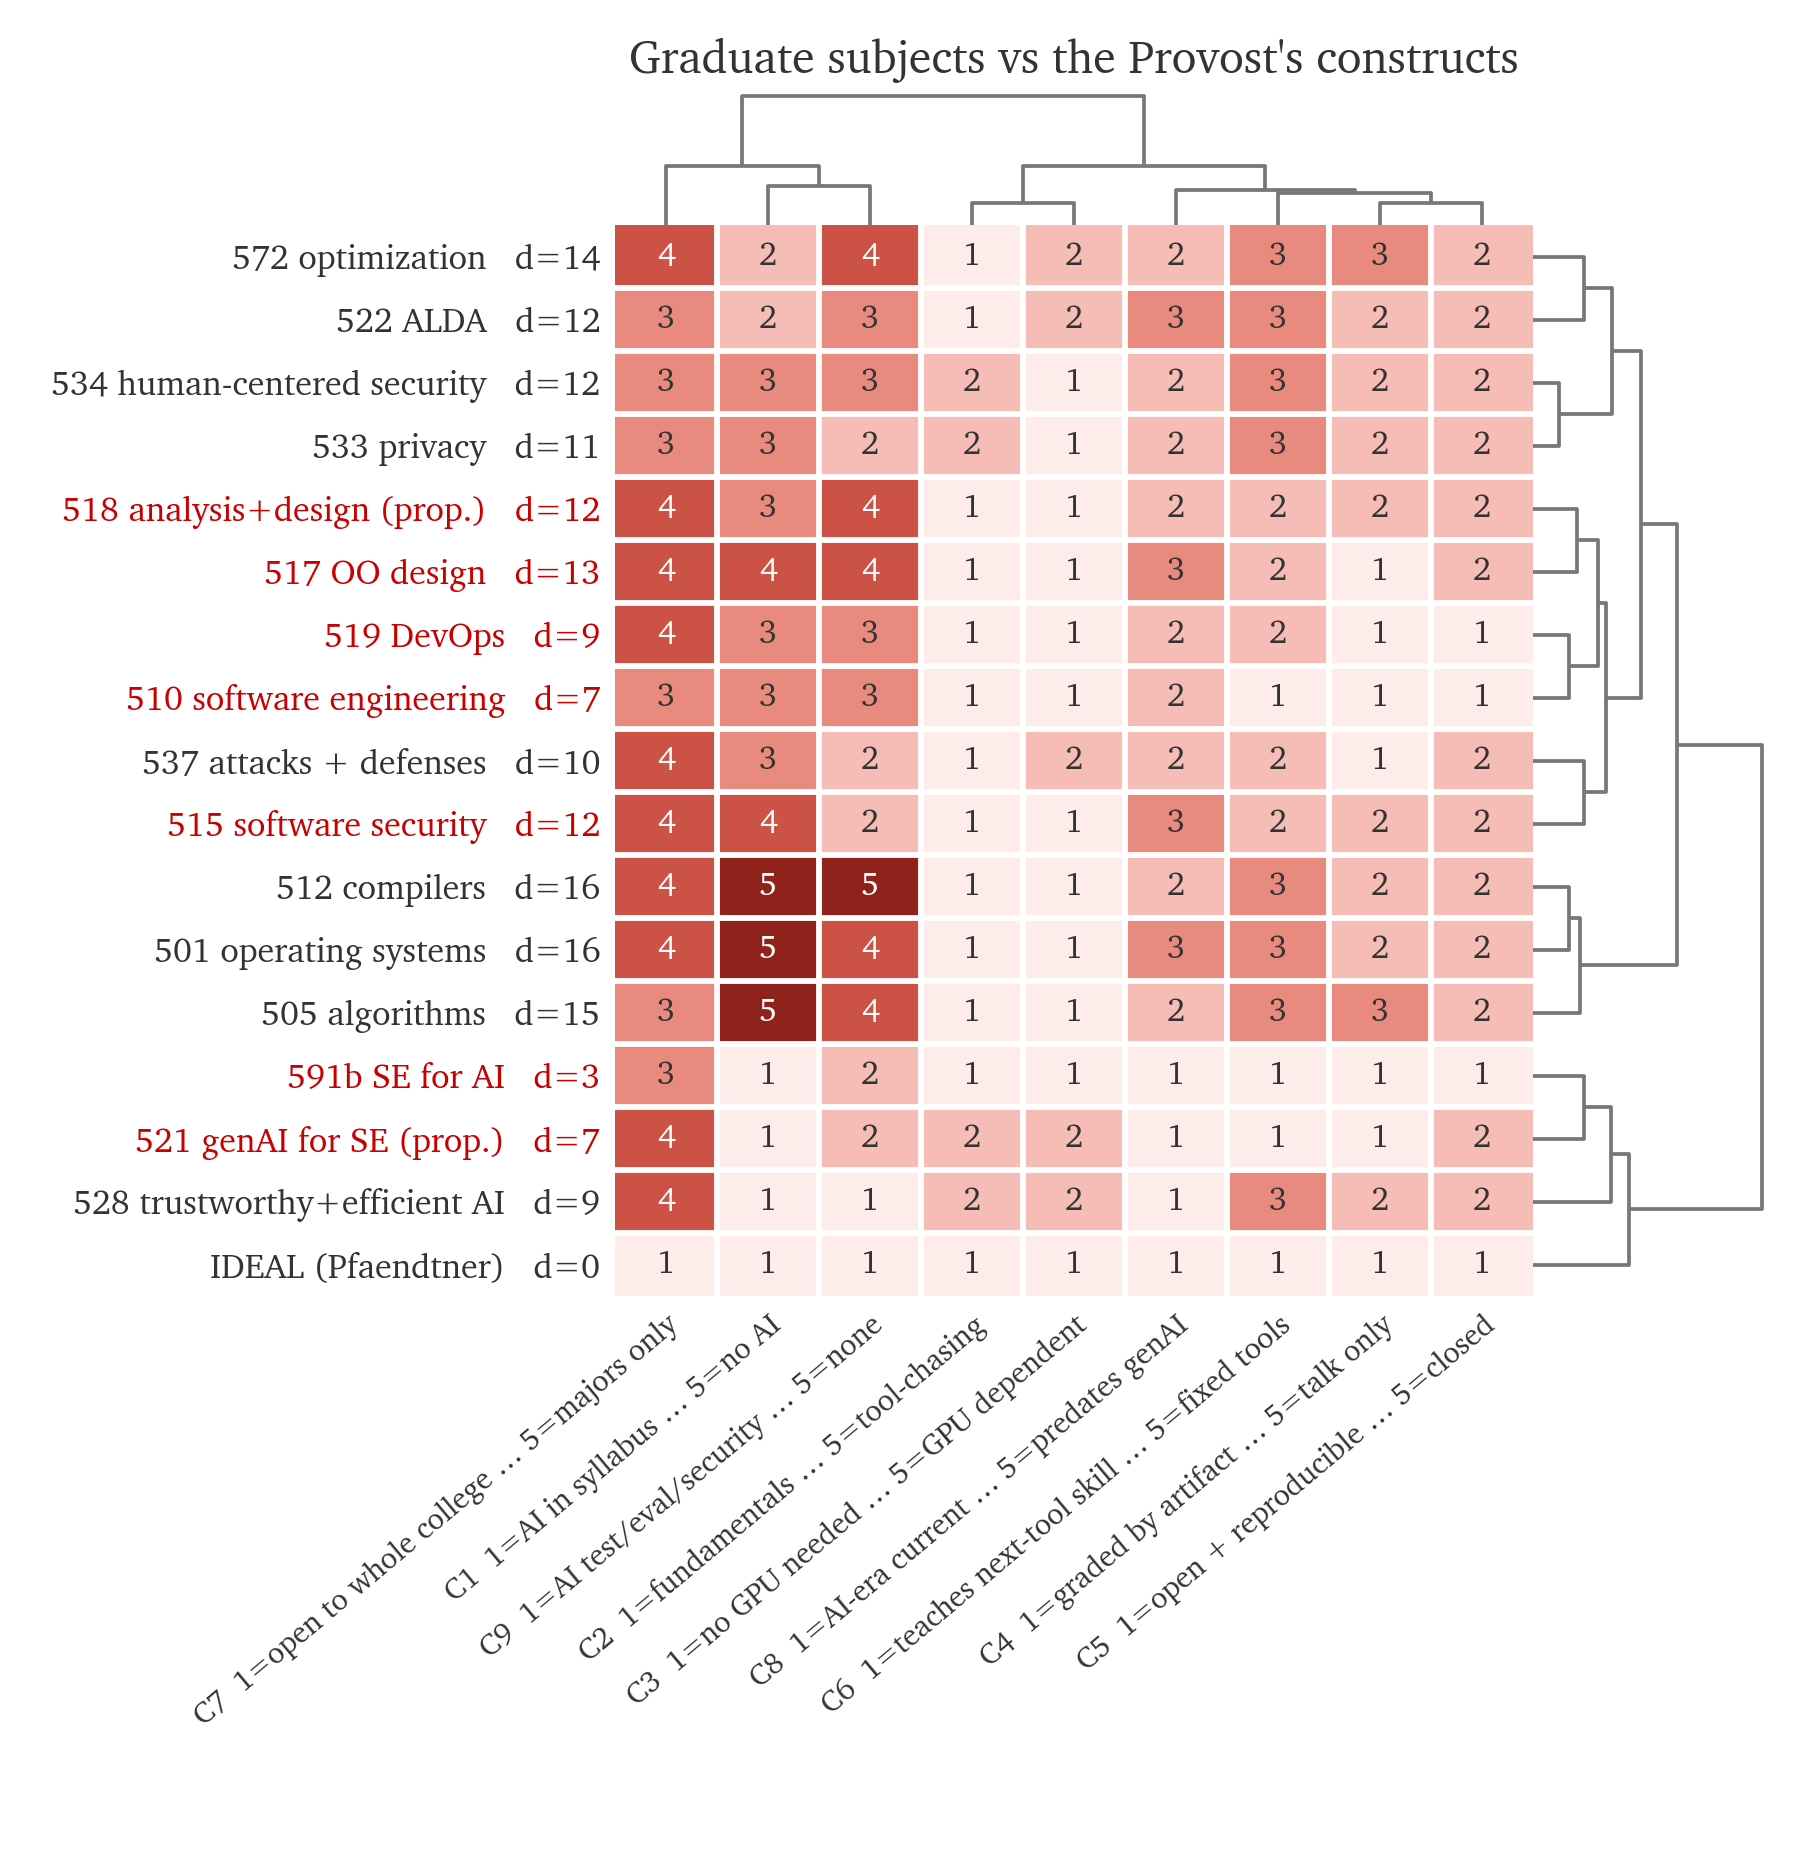
\includegraphics[width=0.80\textwidth]{grad-grid.png}
\end{center}
\vspace{-8pt}

{\footnotesize FOCUS-style clustered grid: dendrograms above (constructs) and right (subjects). \se{Red labels} are SE subjects.}

\textbf{Three reads.} \textbf{(i) The graduate grid repeats the undergraduate shape.} The branch nearest IDEAL holds \se{591b} (d=3), \se{521} (d=7), and 528 (d=9), with \se{510} (d=7) and \se{519} (d=9) on the next branch. The near-approved MS+AI core does not need new inventions. Its closest-to-ideal subjects already run, or sit one paperwork step away. \textbf{(ii) C7 is the graduate weakness.} Most graduate subjects score 3--4 on serves-the-whole-college. This is structural, not a defect: graduate courses carry prerequisites. The grid states the division of labor plainly --- the graduate catalog supplies depth; the freshman 202/301 sequence supplies reach. We should not promise the Provost college-wide service from the graduate program. \textbf{(iii) The theory trio mirrors undergrad.} 501, 505, and 512 (d=15--16) score a perfect 1 on fundamentals and near-worst on AI dose and AI assessment. As before: not problems, redose targets.

\textbf{One methods note, from verification.} We scored \se{510} two ways. Its catalog entry alone gives a distance near 12. Its live Fall 2026 repository --- open course materials, tool talks, an AI-for-SE night, a project that maintains code the students did not write --- gives d=7. The lesson generalizes: score courses as taught, not as cataloged. That is why every cell in these grids must be checked with the lecturer before this memo leaves the building.

\end{document}
